\documentclass[compress,xcolor=table,11pt]{beamer}

% Packages
\usepackage[english, french]{babel}
\usepackage[utf8]{inputenc}
\usepackage[T1]{fontenc}
\usepackage{datetime}
\usepackage{longtable}
\usepackage{booktabs}
\usepackage{wrapfig}
\usepackage{array}
\usepackage{setspace}

\usepackage{float} % add option H for table
\usepackage{subcaption} % add subfigure and subcaption, see package options

% Possible options:
%  - nosectionpages: no pages between sections
%  - flama: use flama font, requires xelatex/lualatex to compile
%  - compressminiframes: put the heading list bullets indications pages on 1 line
\iffalse
\usepackage{fontspec}
\setmainfont[
    Path           = font/,
    Extension      = .otf,
    Ligatures      = TeX,
    BoldFont       = Flama-Bold,
    ItalicFont     = Flama-BasicItalic,
    BoldItalicFont = Flama-BoldItalic
]{Flama-Light}
\fi
%\usetheme[nosectionpages, flama]{upmc}
\usetheme[nosectionpages]{upmc}

\definecolor{hsrmSec3Comp}{rgb}{1,0.509803922,0}
\definecolor{hsrmSec3CompDark}{rgb}{0.666666667,0.333333333,0}

% Title page
\title{M2CAI Workflow Challenge 2016}
\foottitle{M2CAI Workflow Challenge 2016} % optional, by default same as title
\subtitle{Fine tuning CNN with HMM smoothing} % optional
\date{21th October 2016} %\formatdate{4}{10}{2016}}
\author{Rémi \textsc{Cadène}, Thomas \textsc{Robert}, Nicolas \textsc{Thome}, Matthieu \textsc{Cord}}
\institute{University Pierre and Marie Curie - LIP6 - MLIA}




% Biblatex
\usepackage[backend=bibtex,
style=authoryear,
citestyle=authoryear]{biblatex}
\bibliography{library.bib}
\AtEveryBibitem{%
	\clearfield{urldate}%
	\clearfield{urlday}%
	\clearfield{urlmonth}%
	\clearfield{urlyear}%
	\clearfield{doi}%
	\clearfield{issn}%
	\clearfield{isbn}%
	\clearfield{pagetotal}%
	\clearfield{url}%
	\clearfield{timestamp}%
}
\AtEveryCitekey{\UseBibitemHook}
\renewcommand*{\bibfont}{\footnotesize}
\let\oldcite\cite
\renewcommand{\cite}[1]{[\oldcite{#1}]}

\def\tightlist{}


\begin{document}


\begin{frame}[plain]
	\titlepage
	\setcounter{framenumber}{0}
\end{frame}

\section{Context} \subsection{}\label{}

\begin{frame}{M2CAI Workflow Dataset}
	
		\begin{figure}
		\centering
		\begin{subfigure}{.49\textwidth}
			\centering
			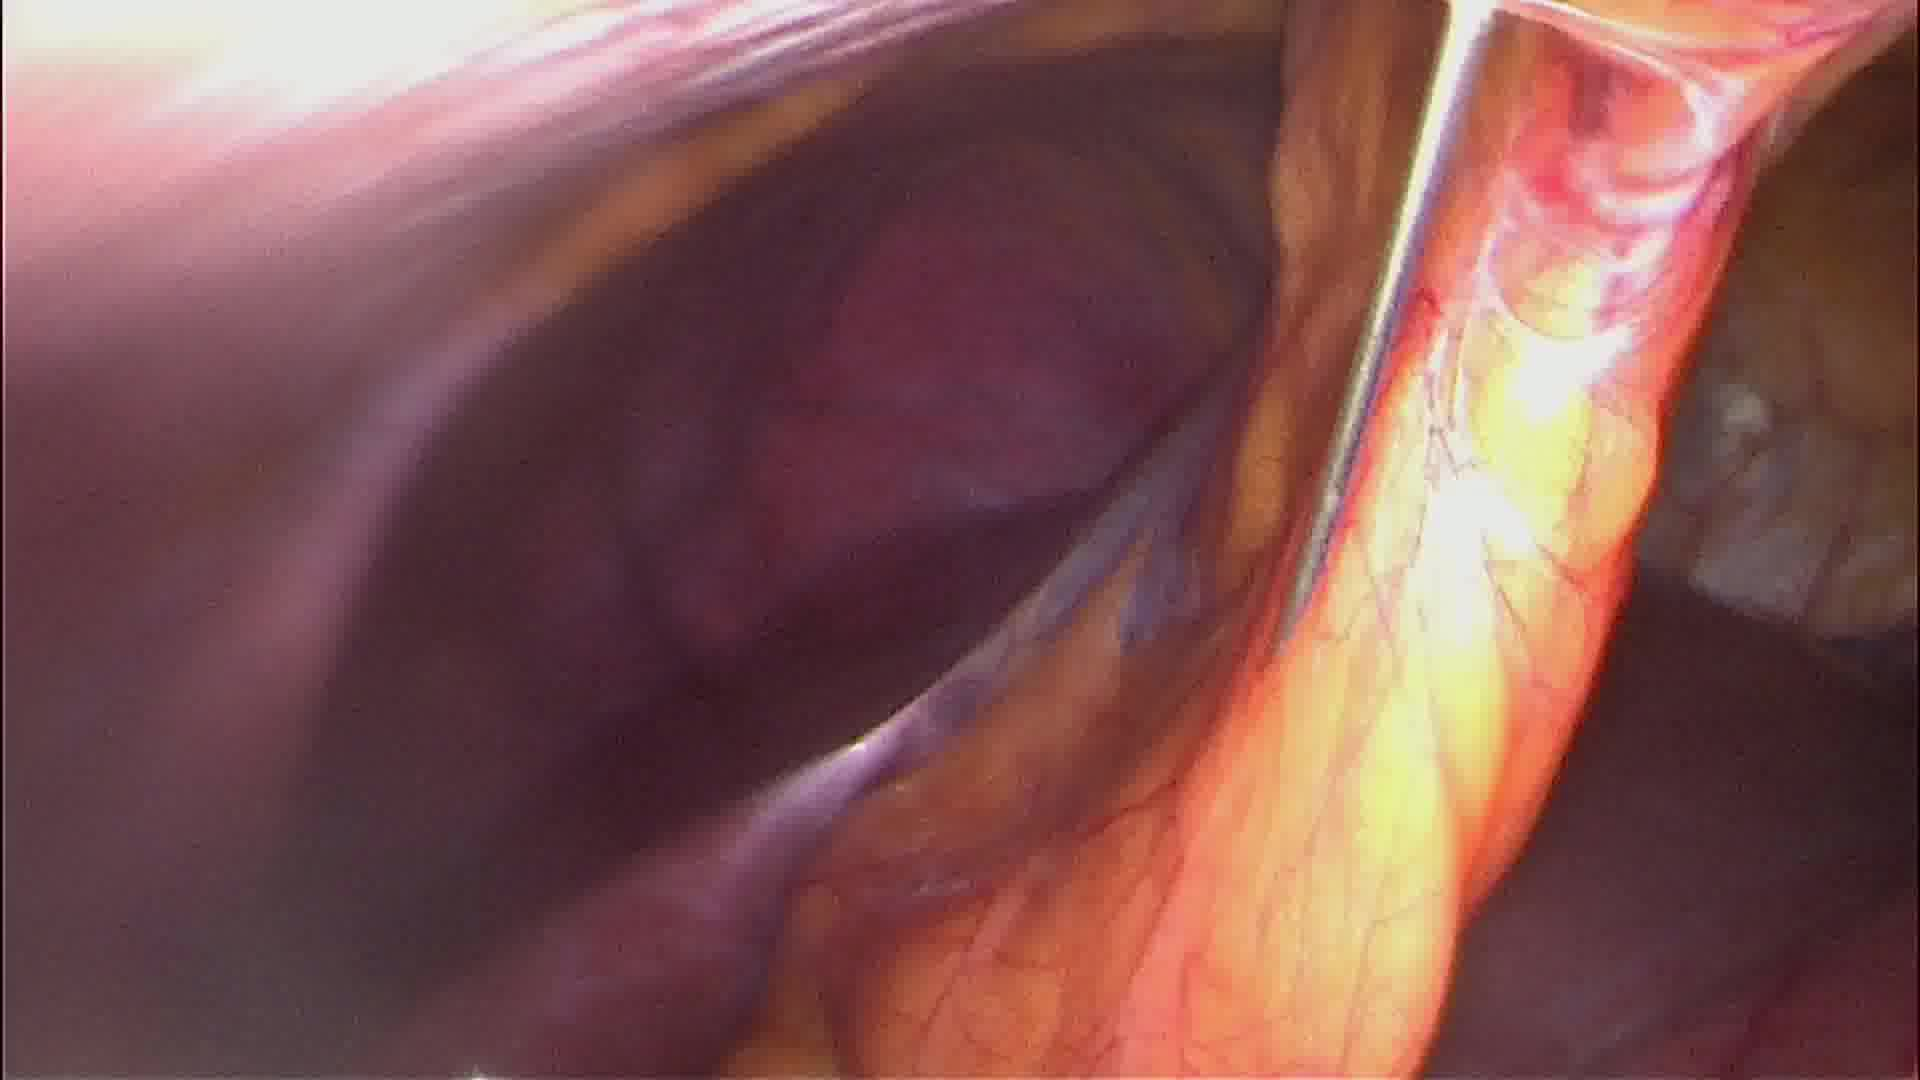
\includegraphics[width=.90\linewidth]{images/m2cai.jpg}
			%			\caption{\small North-South (3479)}
			\label{fig:dsg1}
		\end{subfigure}%
		\begin{subfigure}{.49\textwidth}
			\centering
			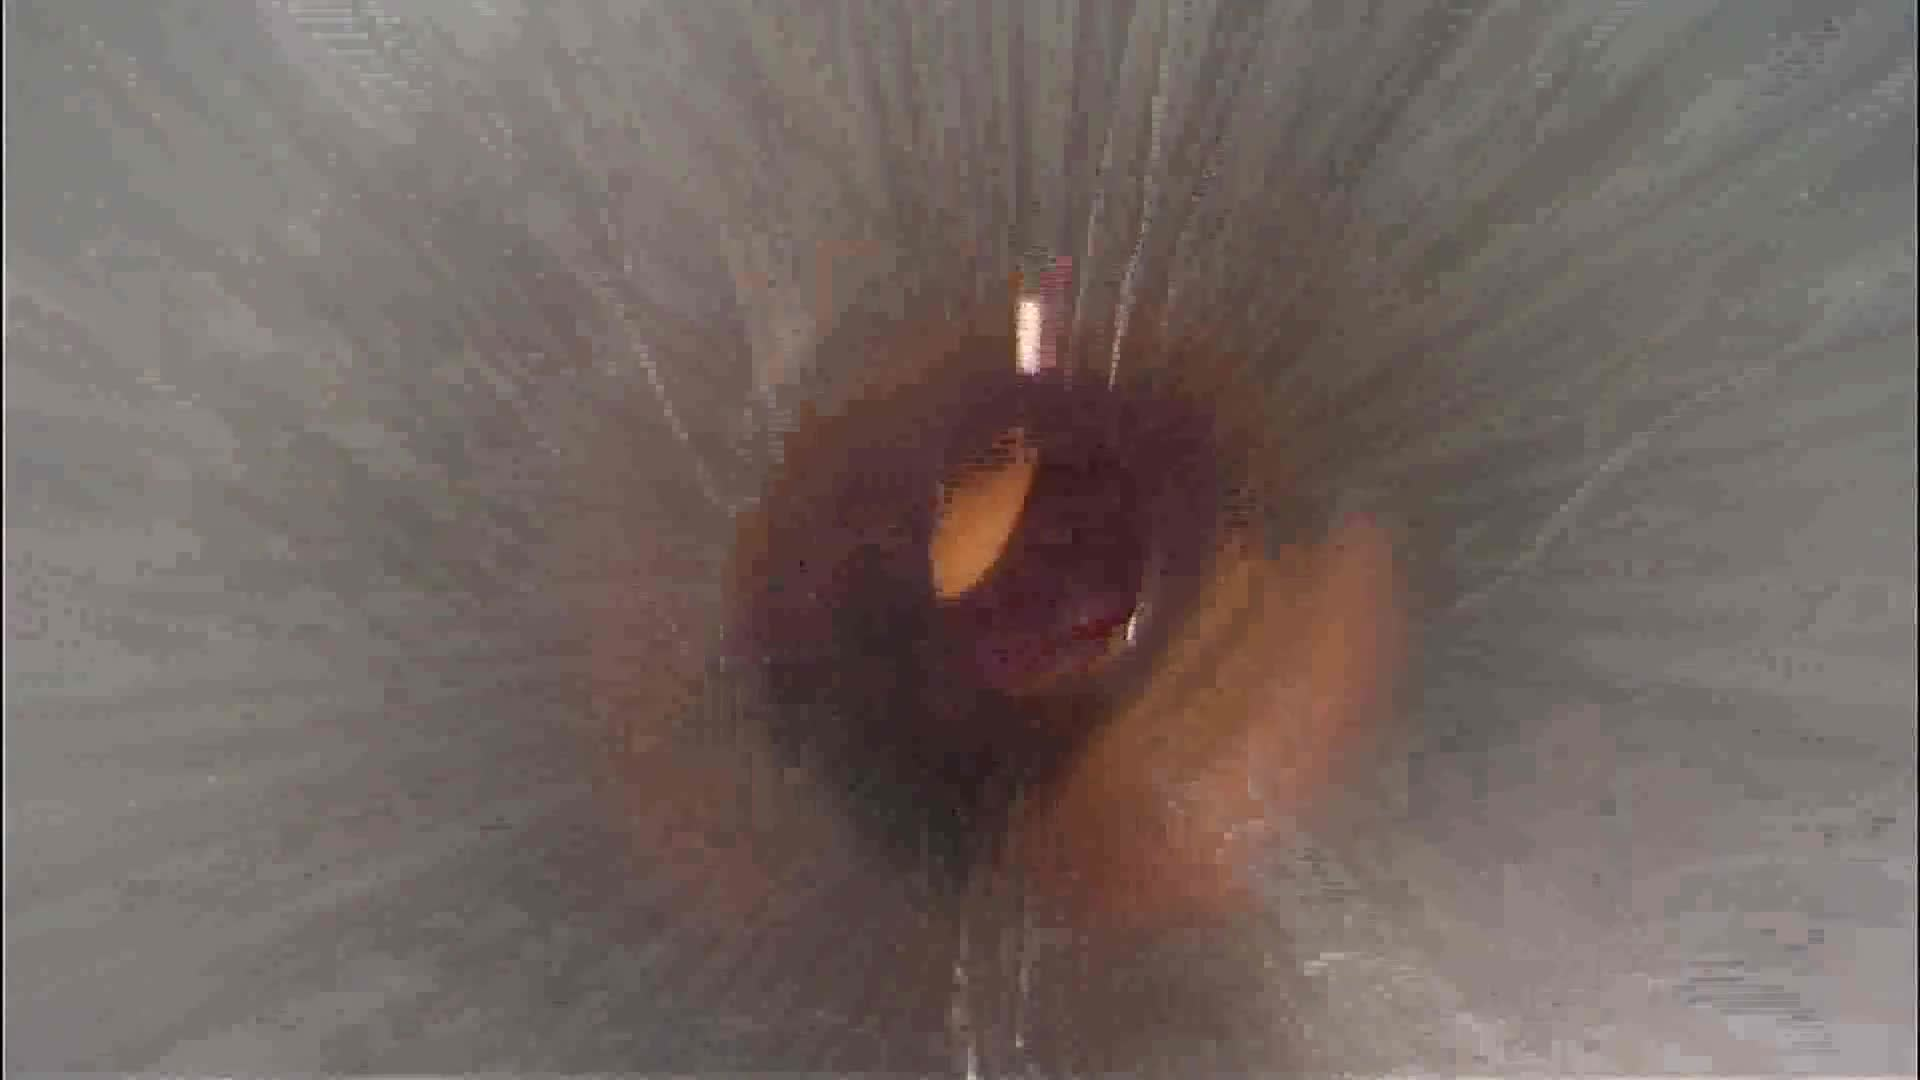
\includegraphics[width=.90\linewidth]{images/m2cai-2.jpg}
			%		\caption{\small East-West (1856)}
			\label{fig:dsg2}
		\end{subfigure}
%		\caption{8000 train images, 20760 no label, 13999 test images}
		\label{fig:dsgimages}
	\end{figure}
	
	Videos resolution is 1920 x 1080, shot at 25 frames per second at the IRCAD research center in Strasbourg, France.
	
	\begin{itemize}
		\item 27 training videos ranging from 15mn to 1hour%(67,595 images)
		%\item 22 train videos %(59,493 images)
		%\item 5 val videos %(8,062 images)
		\item 15 test videos %(28,732 images)
		%\item 8 classes (CleaningCoagulation, CalotTriangleDissection, CLippingCutting, etc.)
	\end{itemize}
	
\end{frame}

\begin{frame}{M2CAI Workflow Dataset}

	1 of 8 classes for each frames:
	\begin{itemize}
		\item TrocarPlacement
		\item Preparation
		\item CalotTriangleDissection
       	\item ClippingCutting
       	\item GallbladderDissection
       	\item GallbladderPackaging
       	\item CleaningCoagulation
       	\item GallbladderRetraction
    \end{itemize}

\end{frame}

\begin{frame}{M2CAI Workflow Goal and Measure}
	
		\begin{block}{Goal}
			\vspace{-.2cm}
	  	\begin{itemize}
	  		\item Online prediction: $P(y | x_i, x_{i-1}, x_{i-2}, ...)$   \\ \hspace{2cm}
	  		$x_i$:= frame $i$, and $y$:= classes
	  	\end{itemize}
		\end{block}
		
		%Detecting at which of the 8 phases of the operation each frames belong.
		
		
		\begin{block}{Useful to}
			\vspace{-.2cm}
		\begin{itemize}
			\item Monitor surgeons
			\item Trigger automatic actions
		\end{itemize}
		\end{block}
		
		\begin{block}{Measures}
						\vspace{-.2cm}
		\begin{itemize}
			\item Jaccard similarity coefficient:
	    $J(A,B) = \frac{| A \cap B |}{| A \cup B|} = \frac{| A \cap B |}{| A| + |B| - |A \cap B|}$
	    
	  		\item Accuracy top1: nb frames well classified / nb total frames
	  	\end{itemize}
	  	\end{block}
		
\end{frame}

\begin{frame}{Two fold approach}

	\begin{block}{1. Frames classifier using Deep Learning}
	\begin{itemize}
		\item From Scratch Convolutional Neural Network (CNN)
		\item Features Extraction CNN 
		\item Fine tuning CNN
	\end{itemize}
	\end{block}
	
	\begin{block}{2. Smoothing predictions}
	\begin{enumerate}	
		\item Averaging predictions over last 15 frames % However, the metric allows a 10 second-margin (not problematic)
		\item Hidden Markov Model (HMM) as a "temporal denoizer" 
	\end{enumerate}
	\end{block}
	
\end{frame}


\section{Frames classifier} \subsection{}\label{}

\begin{frame}{Creating a trainset and valset of images}

	\begin{block}{Creating validation set by random split}
	\begin{itemize}
		\item Training set: 22 videos
		\item Validation set: 5 videos $\{2,9,10,13,27\}$
	\end{itemize}
	\end{block}	
	
	\begin{block}{Extracting one frame every 25 frames (1 frame per second)}
	\begin{itemize}
		\item Training set: 59,493 images
		\item Validation set: 8,062 images
		\item Testing set: 28,732 images
	\end{itemize}
	\end{block}
	

\end{frame}

\begin{frame}{Training CNN From Scratch}

	\begin{figure}[h]
		\centering
		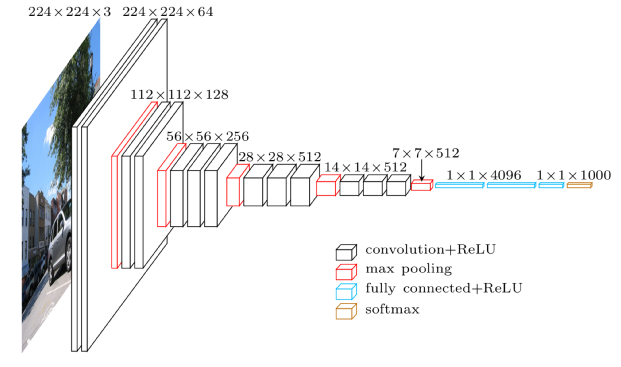
\includegraphics[width=.75\linewidth]{images/vgg16.png}
		\caption{\small Vgg16 \cite{simonyan2014very}, top2 ILSVRC2014}
		\label{fig:quora-invariance-1}
	\end{figure}
	
	\vspace{-.9cm}	
	
	\begin{figure}[h]
		\centering
		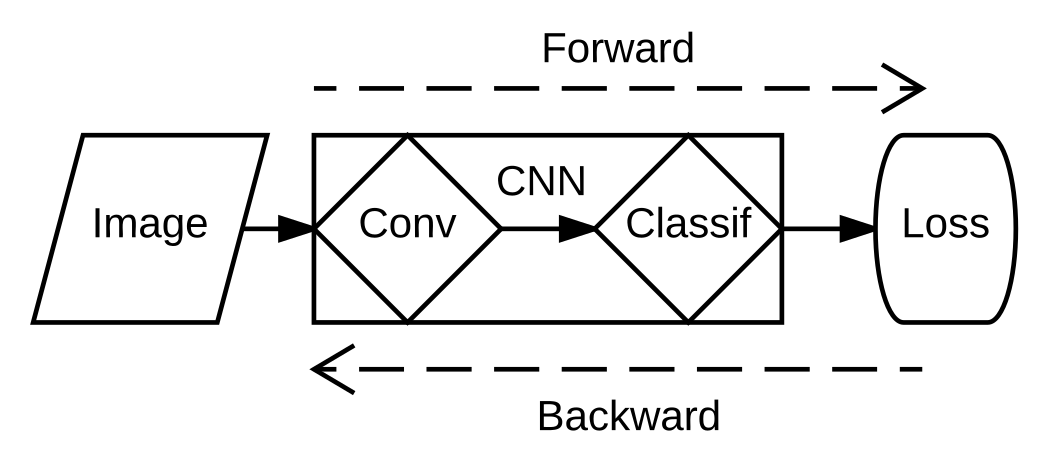
\includegraphics[width=.50\linewidth]{images/FromScratch.png}
		\label{fig:quora-invariance-1}
	\end{figure}
	
\end{frame}

\begin{frame}{ImageNet : 1.2M training images, 1000 classes}
	
	\vspace{-.6cm}
	
	\begin{figure}
		\centering
		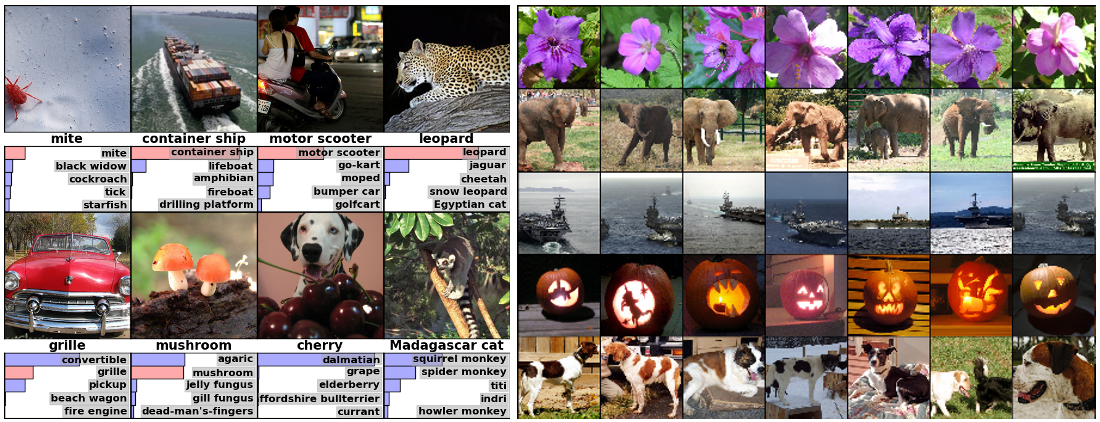
\includegraphics[width=1.04\linewidth]{images/imagenet.png}
		%		\caption{80000 train images, 20000 test images, 101 classes}
		\label{fig:2images}
	\end{figure}
	
	\vspace{-.5cm}
		
	\begin{figure}[h]
		\centering
		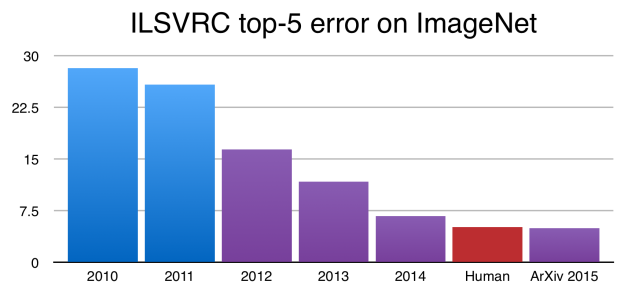
\includegraphics[width=.65\linewidth]{images/ILSVRC.png}
		\label{fig:quora-invariance-1}
	\end{figure}

\end{frame}

\begin{frame}{Using representations learned on ImageNet}
	
	\begin{block}{\small Pre-trained CNN as Features Extractor}
		\vspace{-.2cm}
	\begin{enumerate}
		\item Extracting features somewhere
		\item Training a Support Vector Machine
	\end{enumerate}
	\end{block}
	
		\vspace{-.2cm}
		
	\begin{figure}
		\centering
		\begin{subfigure}{.59\textwidth}
			\centering
			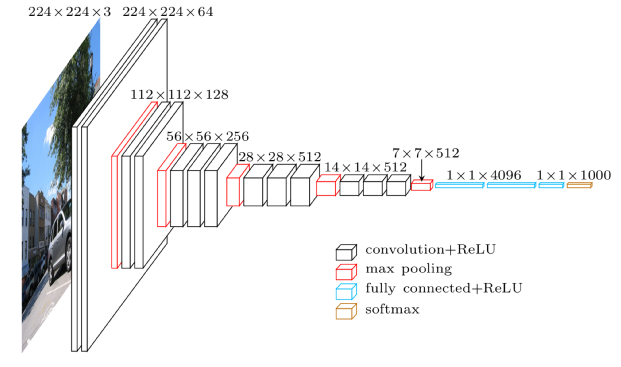
\includegraphics[width=.99\linewidth]{images/vgg16.png}
			%			\caption{\small North-South (3479)}
			\label{fig:dsg1}
		\end{subfigure}%
		\begin{subfigure}{.39\textwidth}
			\centering
			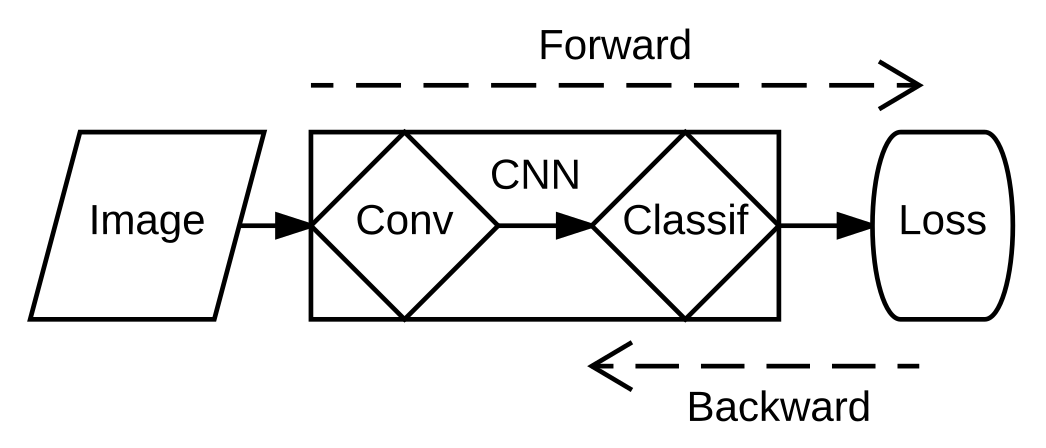
\includegraphics[width=.99\linewidth]{images/Extraction.png}
			%		\caption{\small East-West (1856)}
			\label{fig:dsg2}
		\end{subfigure}
%		\caption{8000 train images, 20760 no label, 13999 test images}
		\label{fig:dsgimages}
	\end{figure}	
	

\end{frame}


\begin{frame}{Adapting representations learned on Imagenet}

	\begin{block}{\small Fine tuning a pre-trained CNN}
		\vspace{-.2cm}
	\begin{itemize}
		\item Same process than CNN From Scratch
		\item But smaller learning rate for pre-trained layers
	\end{itemize}
	\end{block}
	
		\vspace{-.2cm}
	
	\begin{figure}
		\centering
		\begin{subfigure}{.59\textwidth}
			\centering
			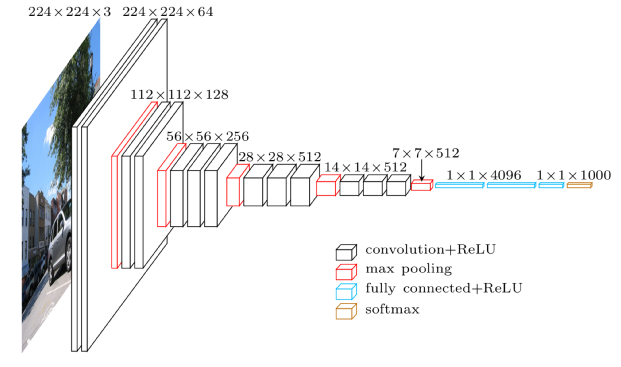
\includegraphics[width=.99\linewidth]{images/vgg16.png}
			%			\caption{\small North-South (3479)}
			\label{fig:dsg1}
		\end{subfigure}%
		\begin{subfigure}{.39\textwidth}
			\centering
			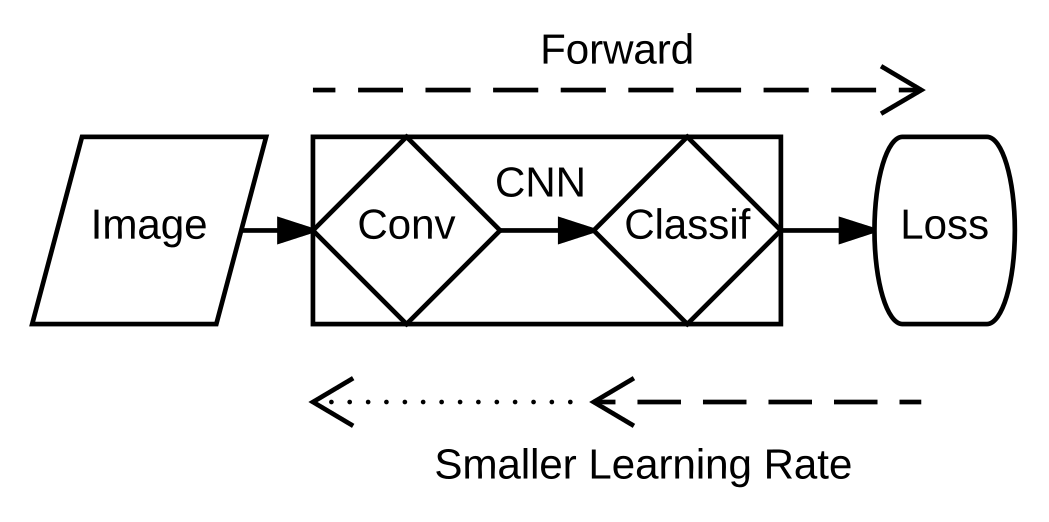
\includegraphics[width=.99\linewidth]{images/FineTuning.png}
			%		\caption{\small East-West (1856)}
			\label{fig:dsg2}
		\end{subfigure}
%		\caption{8000 train images, 20760 no label, 13999 test images}
		\label{fig:dsgimages}
	\end{figure}	

\end{frame}

\begin{frame}{Which CNN to use ? Possible in production ?}

		\begin{table}[h]
		\centering
		\resizebox{300pt}{!}{%
			\begin{tabular}{|c|c|c|c|c|c|c|}
				\hline
				Model & Input & Param. & Depth & Implem. & Forward (ms) & Backward (ms) \\ \hline \hline
				Vgg16 & 224 & 138M & 16 & GPU & 185.29 & 437.89 \\
				InceptionV3 & 399 & 24M & 42 & GPU & \textbf{102.21} & 311.94\\
				ResNet-200  & 224 & 65M & 200 & GPU & 273.85 & 687.48\\ \hline
				InceptionV3 & 399 & 24M & 42 & CPU & 19918.82 & 23010.15 \\
				\hline
			\end{tabular}}
			\caption{\small Forward+Backward with batches of 20 images.} 
			\label{table:cnnbenchmark}
		\end{table}
		
		\textbf{Possible in production thanks to GPUs !}

\end{frame}

\begin{frame}{Comparison of frames classifiers}
	
	\begin{table}
	\begin{center}
				\resizebox{300pt}{!}{%
		\begin{tabular}{|c|c|c|}
			\hline
			Model & Type & Accuracy (\%) \\
			\hline\hline
			InceptionV3 & Extraction (repres. of ImageNet)& 60.53 \\
			InceptionV3 & From Scratch (repres. of M2CAI) & 69.13 \\
			%InceptionV3 Weldon & 78.18 \\
			InceptionV3 & Fine-tuning (both representations) & 79.06 \\
			\textbf{ResNet200} & \textbf{Fine-tuning (both representations)} & \textbf{79.24} \\
			\hline
		\end{tabular}}
	\end{center}
	\caption{Accuracy on the validation set.}
	\end{table}

	\begin{figure}
		\centering
		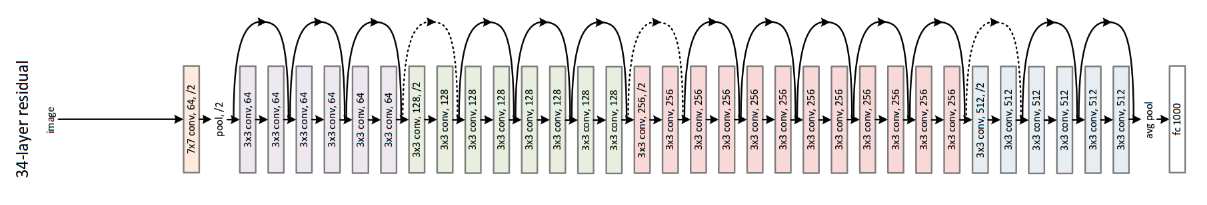
\includegraphics[width=1\linewidth]{images/resnet.png}
		%		\caption{80000 train images, 20000 test images, 101 classes}
		\label{fig:2images}
	\end{figure}
	


\end{frame}


\section{Smoothing predictions} \subsection{}\label{}

\begin{frame}{Gaussian Hidden Markov Model}
	
	\begin{block}{HMM on the smoothed predictions over last 15 frames}
		\vspace{-.2cm}
	\begin{itemize}
		\item Initial state probabilities
		\item Matrix of probabilities of transition between states 
		\item Gaussian parameters for emissions of observations : \\
		\hspace{4cm} -> mean and co-variance matrix
	\end{itemize}
	\end{block}	
	
	\begin{figure}
		\centering
		\begin{subfigure}{.49\textwidth}
			\centering
			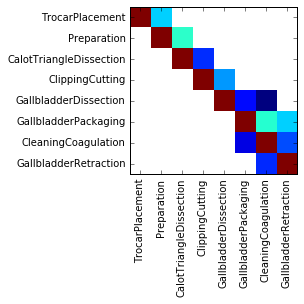
\includegraphics[width=.75\linewidth]{images/index.png}
			%			\caption{\small North-South (3479)}
			\label{fig:dsg1}
		\end{subfigure}%
		\begin{subfigure}{.49\textwidth}
			\centering
			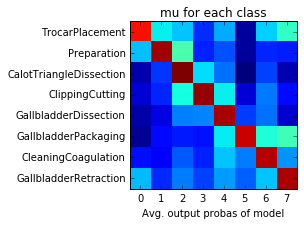
\includegraphics[width=.90\linewidth]{images/index2.png}
			%		\caption{\small East-West (1856)}
			\label{fig:dsg2}
		\end{subfigure}
%		\caption{8000 train images, 20760 no label, 13999 test images}
		\label{fig:dsgimages}
	\end{figure}	
	
\end{frame}

\begin{frame}{Gaussian Hidden Markov Model}
	
	\begin{block}{Training process}
		\begin{itemize}
			\item Counting, Counting
			\item Counting
		\end{itemize}
	\end{block}
	
	\begin{block}{Testing process}
		\begin{itemize}
			\item Offline testing : Viterbi algorithm to obtain the most likely sequence of states
			\item Online testing : to predict $x_t$ we apply Viterbi on the sequence $y_1,...,y_t$
		\end{itemize}
	\end{block}

\end{frame}
	

\begin{frame}{Comparison of temporal smoothing methods}

	\begin{table}
	\begin{center}
		\resizebox{300pt}{!}{%
		\begin{tabular}{|c|c|c|c|}
			\hline
			Temporal Method & Accuracy Val (\%) & Jaccard Val & Jaccard Test \\
			\hline\hline
			No Smoothing & 79.24 & -- & -- \\
			Avg Smoothing & 85.97 & 74.67 & -- \\
			\textbf{Avg + HMM Online} & \textbf{88.90} & \textbf{81.60} & \textbf{71.9} \\ \hline
			Avg + HMM Offline & 93.47 & 87.59 & -- \\
			\hline
		\end{tabular}}
	\end{center}
	\caption{With the predictions of our fine tuned ResNet-200}
	\end{table}

\end{frame}

\begin{frame}{Visualization}

	\begin{figure}
\begin{center}
%\fbox{\rule{0pt}{2in} \rule{0.9\linewidth}{0pt}}
   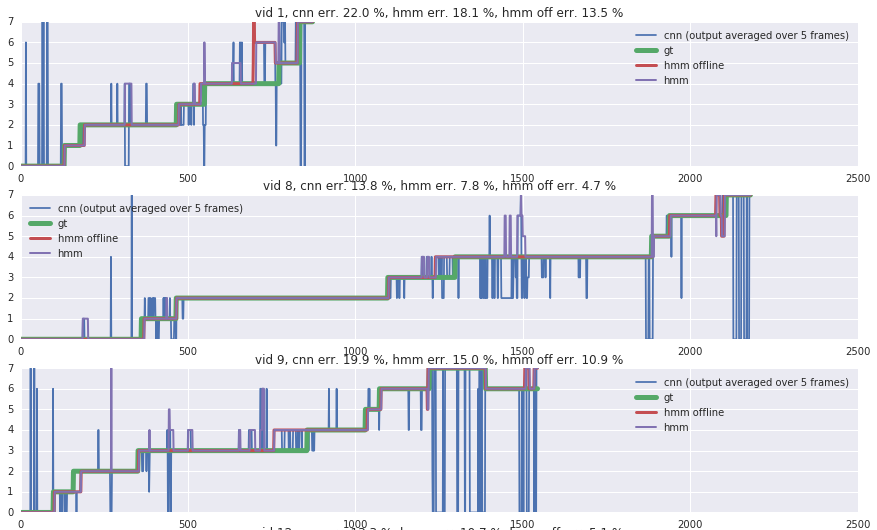
\includegraphics[width=1\linewidth]{images/visu1.png}
\end{center}
\label{fig:long}
\label{fig:onecol}
\end{figure}	
	
\end{frame}

\begin{frame}{Visualization}
	
	\begin{figure}
		\begin{center}
			%\fbox{\rule{0pt}{2in} \rule{0.9\linewidth}{0pt}}
			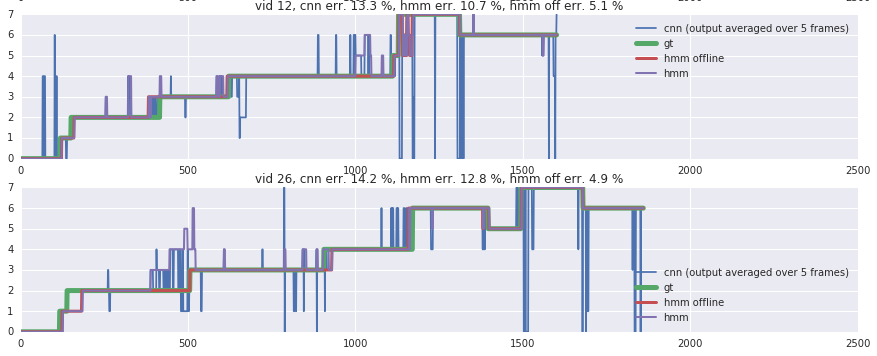
\includegraphics[width=1\linewidth]{images/visu2.png}
		\end{center}
		\label{fig:long}
		\label{fig:onecol}
	\end{figure}	
	
\end{frame}


\section{Conclusion} \subsection{}\label{}

\begin{frame}{Conclusion}

	\begin{block}{Conclusion}
		\begin{itemize}
			\item Deep Learning efficient %to takle this problem
			\item Fine Tuning most accurate approach %to build a frames classifier
			\item HMM is usefull to smooth the predictions %to add a prior in order to smooth the predictions
		\end{itemize}
	\end{block}
	
	\begin{block}{Future work}
		\begin{itemize}
			\item Fine tuning CNN on full trainset (not only 80\%)
			\item Ensembling several fine tuned CNNs
		\end{itemize}
	\end{block}
	
	Code available: \url{github.com/Cadene/torchnet-m2caiworkflow}
	
\end{frame}

\section{References} \subsection{}\label{references}

\begin{frame}[allowframebreaks]{References}
	
	\printbibliography[heading=none]
	
\end{frame}


\end{document}
